\section{FFOps\_\-OL\_\-neu Class Reference}
\label{classFFOps__OL__neu}\index{FFOps_OL_neu@{FFOps\_\-OL\_\-neu}}
This class is inherited from class {\tt FF\_\-Basic\_\-neu} for mutations on a network. 


{\tt \#include $<$FFOps\_\-OL\_\-neu.h$>$}

Inheritance diagram for FFOps\_\-OL\_\-neu::\begin{figure}[H]
\begin{center}
\leavevmode
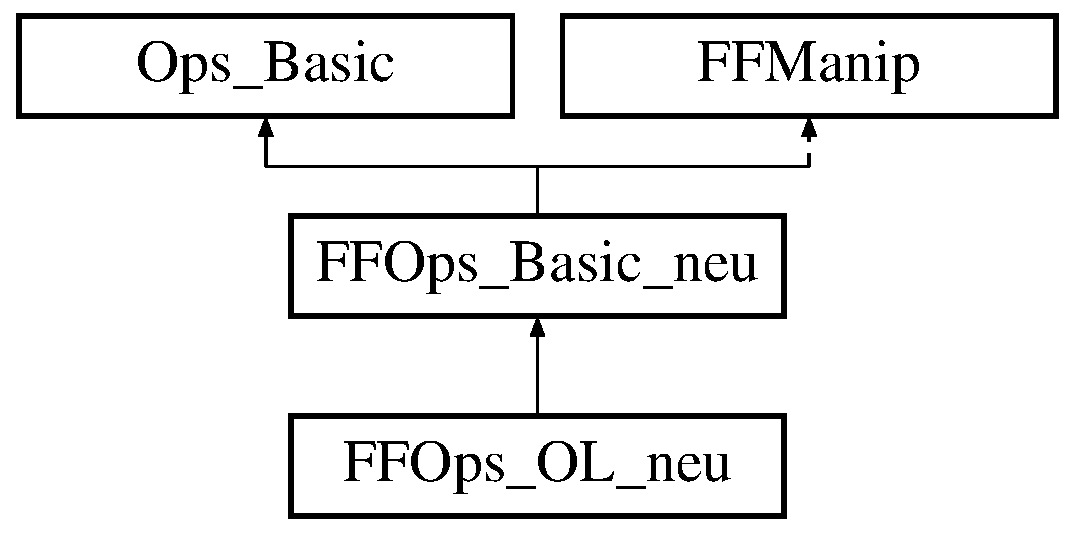
\includegraphics[height=3cm]{classFFOps__OL__neu}
\end{center}
\end{figure}
\subsection*{Public Methods}
\begin{CompactItemize}
\item 
void {\bf init\-Connections} (Individual \&Ind, double prob1=1.0, double prob2=1.0, double prob3=1.0)
\begin{CompactList}\small\item\em Modify weights of a layered network.\item\end{CompactList}\item 
void {\bf add\-Connection} (Individual \&Ind, double low, double high)
\begin{CompactList}\small\item\em Add connections where possible and initialize the weight.\item\end{CompactList}\item 
void {\bf delete\-Connection} (Individual \&Ind, const double sigma=-1)
\begin{CompactList}\small\item\em delete a connection\item\end{CompactList}\item 
void {\bf delete\-Neuron} (Individual \&Ind)
\begin{CompactList}\small\item\em delete a neuron\item\end{CompactList}\item 
void {\bf add\-Neuron} (Individual \&Ind, double low, double high)
\begin{CompactList}\small\item\em Add a neuron.\item\end{CompactList}\item 
\index{deleteNeuronGain@{deleteNeuronGain}!FFOps_OL_neu@{FFOps\_\-OL\_\-neu}}\index{FFOps_OL_neu@{FFOps\_\-OL\_\-neu}!deleteNeuronGain@{deleteNeuronGain}}
void {\bf delete\-Neuron\-Gain} (Individual \&Ind, double sigma=-1)\label{classFFOps__OL__neu_a5}

\begin{CompactList}\small\item\em Delete the output of a neuron.\item\end{CompactList}\item 
\index{deleteNeuronActivation@{deleteNeuronActivation}!FFOps_OL_neu@{FFOps\_\-OL\_\-neu}}\index{FFOps_OL_neu@{FFOps\_\-OL\_\-neu}!deleteNeuronActivation@{deleteNeuronActivation}}
void {\bf delete\-Neuron\-Activation} (Individual \&, double=-1)\label{classFFOps__OL__neu_a6}

\begin{CompactList}\small\item\em Delete the activation of a neuron.\item\end{CompactList}\end{CompactItemize}


\subsection{Detailed Description}
This class is inherited from class {\tt FF\_\-Basic\_\-neu} for mutations on a network.



\subsection{Member Function Documentation}
\index{FFOps_OL_neu@{FFOps\_\-OL\_\-neu}!addConnection@{addConnection}}
\index{addConnection@{addConnection}!FFOps_OL_neu@{FFOps\_\-OL\_\-neu}}
\subsubsection{\setlength{\rightskip}{0pt plus 5cm}void FFOps\_\-OL\_\-neu::add\-Connection (Individual \& {\em Ind}, double {\em low}, double {\em high})}\label{classFFOps__OL__neu_a1}


Add connections where possible and initialize the weight.

\begin{Desc}
\item[Parameters: ]\par
\begin{description}
\item[{\em 
Ind}]representing the network in which connection to be added \item[{\em 
low:}]lower bound of the interval for generating a random weight \item[{\em 
high:}]upper bound of the interval for generating a random weight \end{description}
\end{Desc}
\index{FFOps_OL_neu@{FFOps\_\-OL\_\-neu}!addNeuron@{addNeuron}}
\index{addNeuron@{addNeuron}!FFOps_OL_neu@{FFOps\_\-OL\_\-neu}}
\subsubsection{\setlength{\rightskip}{0pt plus 5cm}void FFOps\_\-OL\_\-neu::add\-Neuron (Individual \& {\em Ind}, double {\em low}, double {\em high})}\label{classFFOps__OL__neu_a4}


Add a neuron.

Add connections between the newly generated neuron and input, output  neurons. Initialize the weights randomly with a given interval. \begin{Desc}
\item[Parameters: ]\par
\begin{description}
\item[{\em 
Ind:}]individual representing the network to be processed \item[{\em 
low:}]lower bound of the interval for generating a random weight \item[{\em 
high:}]upper bound of the interval for generating a random weight \end{description}
\end{Desc}
\index{FFOps_OL_neu@{FFOps\_\-OL\_\-neu}!deleteConnection@{deleteConnection}}
\index{deleteConnection@{deleteConnection}!FFOps_OL_neu@{FFOps\_\-OL\_\-neu}}
\subsubsection{\setlength{\rightskip}{0pt plus 5cm}void FFOps\_\-OL\_\-neu::delete\-Connection (Individual \& {\em Ind}, const double {\em sigma} = -1)}\label{classFFOps__OL__neu_a2}


delete a connection

\begin{Desc}
\item[Parameters: ]\par
\begin{description}
\item[{\em 
Ind}]representing the network in which a connection is to be deleted  \item[{\em 
sigma}]? \end{description}
\end{Desc}
\index{FFOps_OL_neu@{FFOps\_\-OL\_\-neu}!deleteNeuron@{deleteNeuron}}
\index{deleteNeuron@{deleteNeuron}!FFOps_OL_neu@{FFOps\_\-OL\_\-neu}}
\subsubsection{\setlength{\rightskip}{0pt plus 5cm}void FFOps\_\-OL\_\-neu::delete\-Neuron (Individual \& {\em Ind})}\label{classFFOps__OL__neu_a3}


delete a neuron

\begin{Desc}
\item[Parameters: ]\par
\begin{description}
\item[{\em 
Ind}]representing the network in which a neuron is to be deleted \end{description}
\end{Desc}
\index{FFOps_OL_neu@{FFOps\_\-OL\_\-neu}!initConnections@{initConnections}}
\index{initConnections@{initConnections}!FFOps_OL_neu@{FFOps\_\-OL\_\-neu}}
\subsubsection{\setlength{\rightskip}{0pt plus 5cm}void FFOps\_\-OL\_\-neu::init\-Connections (Individual \& {\em Ind}, double {\em prob1} = 1.0, double {\em prob2} = 1.0, double {\em prob3} = 1.0)}\label{classFFOps__OL__neu_a0}


Modify weights of a layered network.

\begin{Desc}
\item[Parameters: ]\par
\begin{description}
\item[{\em 
Ind}]representing the network to be modified \item[{\em 
prob1:}]probability for a connection between input and hidden nodes \item[{\em 
prob2:}]probability for a connection between hidden and output nodes \item[{\em 
prob3:}]probability for a connection between bias nodes and other nodes \end{description}
\end{Desc}


The documentation for this class was generated from the following file:\begin{CompactItemize}
\item 
FFOps\_\-OL\_\-neu.h\end{CompactItemize}
